\documentclass[slidestop,compress,mathserif]{beamer}

\mode<article> % 仅应用于article版本
{
  \usepackage{beamerbasearticle}
  \usepackage{fullpage}
  \usepackage{hyperref}
}

%% 下面的包控制beamer的风格,可以根据自己的爱好修改
\usepackage{beamerthemesplit}   % 使用split风格
\usepackage{beamerthemeshadow}  % 使用shadow风格
%\usepackage[width=2cm,dark,tab]{beamerthemesidebar}
\usepackage{beamerthemetree}
%\usetheme{Montpellier}
%\usecolortheme{lily}


%% 这些包是可能会用到的,不必修改
\usepackage{amsmath,amssymb}
\usepackage{graphicx}
%\usepackage{color}
%\usepackage{pgf,pgfarrows,pgfnodes,pgfautomata,pgfheaps}
%\usepackage{multimedia}

\begin{document}

%%
%% 填写作者,单位,日期,标题等文档信息
%%
%%%%%%%%%%%%%%%%%%%%%%%%%%%%%%%%%%%%%%%%%%%%%%%%%%%%%%%%%%%%%%%%%%%%%%%%%%%%%%%%%%%%%%%%%%%%%
\title{Algorithm Problem}
%\subtitle{}
\author{Chao, Xiongying, Chunlin, Mingfu, Haicang}
%\institute{}
\date{\today}

%%%%%%%%%%from here by Chao%%%%%%%%%%%%


\frame
{
\frametitle{Pattern Matching -- Problem Statement}
In computer science, $ pattern \  matching$ is the act of checking for the presence of the constituents of a given pattern.
\begin{block}{Formalized Definition:}

{\bf Input: }\\

A target string $T$, a pattern string $P$\\

{\bf Output: }
\begin{itemize}
\item -1 if $T$ has no substring $P$.
\item the first position $i$ of $T$ if $P$ matches the substring of $T$ from position $i$
\end{itemize}

\end{block}
}

\frame
{
\frametitle{Pattern Matching -- Instance}
\begin{block}{Instance 1}
\begin{itemize}
 \item $T\ :\ abbaba$
 \item $P\ :\ aba$
 \item Output: $3.\ $
\item Because $P$ matches the substring of $T$ from position $3$.
\end{itemize}

\end{block}
\begin{block}{Instance 2}
\begin{itemize}
 \item $T\ :\ abbaba$
 \item $P\ :\ abc$
 \item Output: $-1.\ $
\item Because $T$ has no substring $P$.
\end{itemize}


\end{block}

}
\frame
{


\frametitle{Pattern Matching -- Key Observasion}
\begin{itemize}
 \item A trivial method : Enumerate. The time complexity will be $O(mn)$ , in which $m$ means the length of the pattern $P$ and $n$ means the length of the target $T$.
 \item An Improved method : KMP Algorithm.
\end{itemize}

}

\frame
{
\frametitle{Independent Set -- Problem Statement}
In graph theory, an $independent \ set$ or stable set is a set of vertices in a undigraph no two of which are adjacent. 
\begin{block}{Formalized Definition:}

 {\bf Input:}\\

 An undigragh and an integer number $i$.


 {\bf Output:}\\
\begin{itemize}
  \item $1$ if there exits a set of vertices which size is $i$, in the undigragh no two of which have edge.
  \item $0$ for others.
\end{itemize}



\end{block}
}

\frame
{
\frametitle{Independent Set -- Instance}

\begin{figure}
 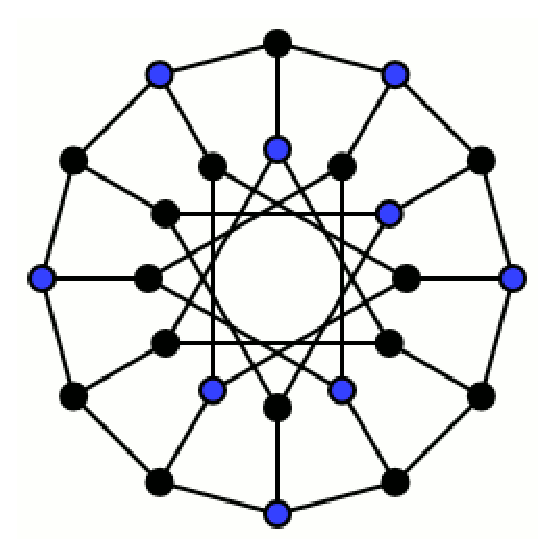
\includegraphics[width=1.5in] {Independent_set_graph.eps}
 % Independent_set_graph.eps: 22002048x0 pixel, 300dpi, 186284.00x0.00 cm, bb=14 14 407 318
\end{figure}

The set of 9 blue vertices is an independent set for this graph of 24 vertices.

}
\frame
{
\frametitle{Independent Set -- Key Observation}
\begin{itemize}
 \item This problem has been proved an $NP$ problem.
 \item A trivial method : Enumerate. The time complexity will be $O(C^i_m)$ , in which $m$ means the number of the vertice.
 \item For some special cases, when $i$ is very small, we can find some Approxiamation Algorithms.
\end{itemize}

}

\frame
{
\frametitle{Stable Matching -- Problem Statement}
In mathematics, the $stable \ marriage \ problem (SMP)$ is the problem of finding a stable matching — a matching in which no element of the first matched set prefers an element of the second matched set that also prefers the first element.
\begin{block}{Formalized Definition:}

 {\bf Input:}\\
$n$ men and $n$ women, where each person has ranked all members of the opposite sex with a unique number between $1$ and $n$ in order of preference.

 {\bf Output:}\\
The matching of the men and women such that there are no two people of opposite sex who would both rather have each other than their current partners. If there are no such people, all the marriages are "stable".



\end{block}
}

\frame
{
\frametitle{Stable Matching -- Instance}
Is matching $X-C,\ Y-B,\ Z-A$ stable?\\
\begin{figure}
 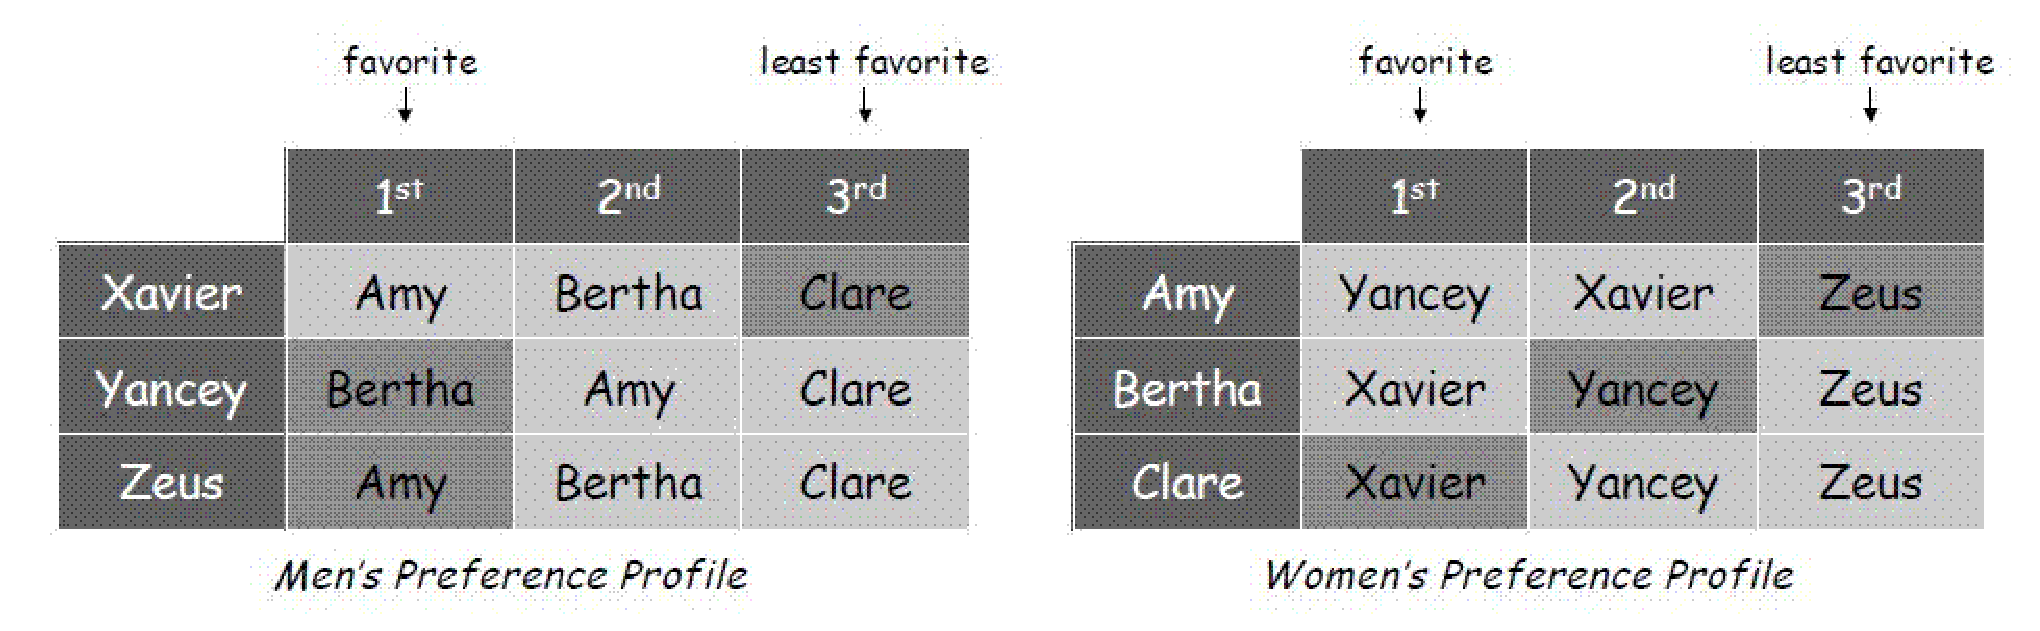
\includegraphics[width=4in] {1.eps}
 % Independent_set_graph.eps: 22002048x0 pixel, 300dpi, 186284.00x0.00 cm, bb=14 14 407 318
\end{figure}


}
\frame
{
\frametitle{Stable Matching -- Instance}
No. Bertha and Xavier will hook up.\\
The matching $X-A,\ Y-B,\ Z-C$ is stable.
}
\frame
{
\frametitle{Stable Matching -- Key Observation}
An Intuitive method that guarantees to find a stable matching:\\
\begin{figure}
 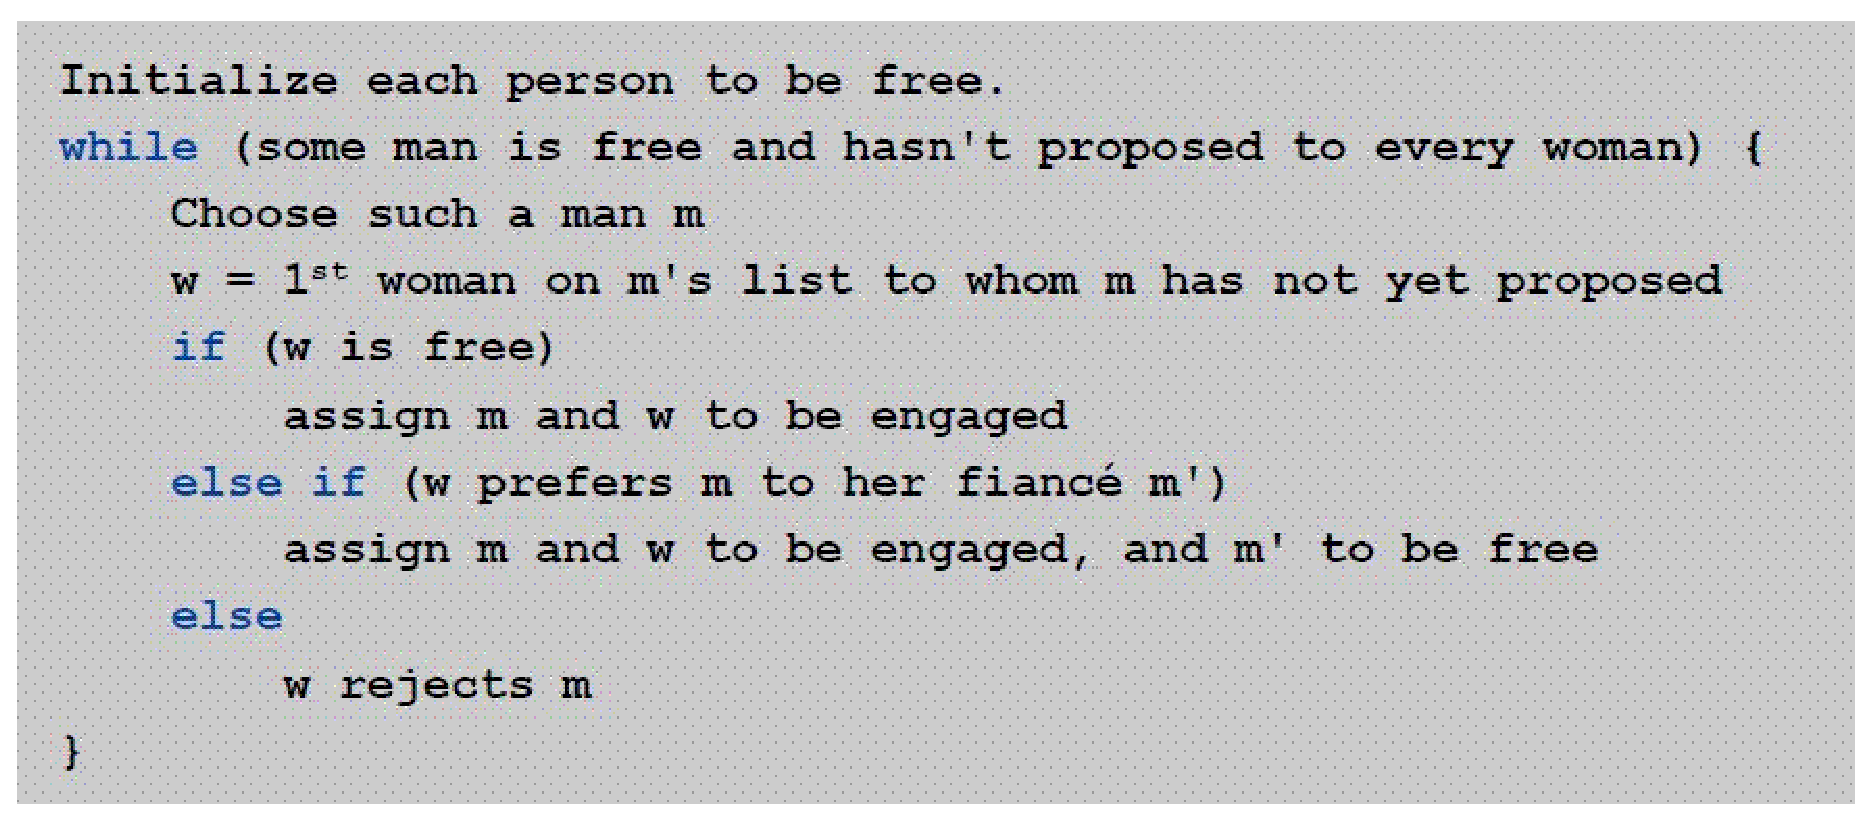
\includegraphics[width=4in] {2.eps}
 % Independent_set_graph.eps: 22002048x0 pixel, 300dpi, 186284.00x0.00 cm, bb=14 14 407 318
\end{figure}
}
\frame
{
\frametitle{Gragh Coloring -- Problem Statement}
In graph theory, $Graph \ Coloring$ is a special case of graph labeling; it is an assignment of labels traditionally called "colors" to elements of a graph subject to certain constraints. In its simplest form, it is a way of coloring the vertices of a graph such that no two adjacent vertices share the same color; this is called a vertex coloring.
\begin{block}{Formalized Definition:}

 {\bf Input: }\\
An undigragh and an integer number $i$

 {\bf Output: }\\
\begin{itemize}
  \item $1$ if there exits a vertex coloring with $i$ colors such that no two adjacent vertices share the same color.
  \item $0$ for others.
\end{itemize}


\end{block}
}

\frame
{
\frametitle{Gragh Coloring -- Instance}
\begin{figure}
 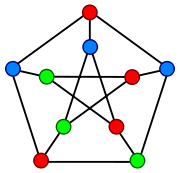
\includegraphics[width=1.5in] {180px-Petersen_graph_3-coloring.svg.eps}
 % Independent_set_graph.eps: 22002048x0 pixel, 300dpi, 186284.00x0.00 cm, bb=14 14 407 318
\end{figure}
A proper vertex coloring of the Petersen graph with $3$ colors, the minimum number possible.
}
\frame
{


\frametitle{Gragh Coloring -- Key Observation}
\begin{itemize}
 \item A trivial method : Greedy Algorithm.
 \item An Approxiamation method : Linear Programming.
\end{itemize}

}
\frame
{
\frametitle{Edge Coloring -- Problem Statement}
In graph theory, an edge coloring of a graph is an assignment of “colors” to the edges of the graph so that no two adjacent edges have the same color. For example, the figure to the right shows an edge coloring of a graph by the colors red, blue, and green. Edge colorings are one of several different types of graph coloring.
\begin{block}{Formalized Definition:}

 {\bf Input: }\\
An undigragh and an integer number $i$

 {\bf Output: }\\
\begin{itemize}
  \item $1$ if there exits a vertex coloring with $i$ colors such that no two adjacent edges share the same color.
  \item $0$ for others.
\end{itemize}


\end{block}
}

\frame
{
\frametitle{Edge Coloring -- Instance}
\begin{figure}
 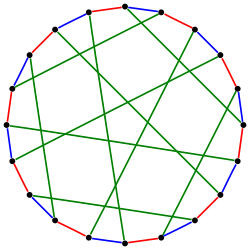
\includegraphics[width=1.5in] {250px-Desargues_graph_3color_edge.svg.eps}
 % Independent_set_graph.eps: 22002048x0 pixel, 300dpi, 186284.00x0.00 cm, bb=14 14 407 318
\end{figure}
3-edge-coloring of Desargues graph.
}
\frame
{


\frametitle{Edge Coloring -- Key Observation}
\begin{itemize}
 \item A trivial method : Greedy Algorithm. (as vertex coloring)
 \item An Approxiamation method : Linear Programming. (as vertex coloring)
\end{itemize}

}
\frame
{
\frametitle{Load Balancing -- Problem Statement}
In computer networking, $Load\  Balancing$ is a technique to distribute workload evenly across two or more computers, network links, CPUs, hard drives, or other resources, in order to get optimal resource utilization, maximize throughput, minimize response time, and avoid overload.\\
We have a set $J$ of $n$ jobs, and a set $M$ of $m$ machines, and the goal is to assign each job to a machine so that the maximum load on any machine will be as small as possible.
}
\frame
{
\frametitle{Load Balancing -- Problem Statement}
\begin{block}{Formalized Definition:}

{ \bf Input: }\\
Each job $j$ has a fixed given size $t_j\geq 0$ and a set of machines $M_j\subseteq M$ that it may be assigned to. The set $M_j$ can be completely arbitrary. We call an assignment of jobs to machines $feasible$ if each job $j$ is assigned to a machine $i\in M_j.$

 {\bf Output: }\\
The goal is still to minimize the maximum load on any machine: Using $J_i\in J$ to denote the jobs assigned to a machine $i\in M$ in a feasible assignment, and using $L_i=\Sigma _{j\in J_i} t_j$ to denote the resulting load, we seek to minimize $max_i L_i$.


\end{block}
}

\frame
{


\frametitle{Load Balancing -- Key Observation}
We can formulate the Load Balancing Problem as a linear program with restrictions on the variable values. Then we can find approximation algorithms for the LP. We have formulated the following problem.
\begin{block}{Linear Programming Formulation}
 $$min L$$
$$\Sigma _i x_{ij} =t_j\ \ for\  all\  i\in J$$
$$\Sigma _j x_{ij} \leq L\ \ for \ all\ i\in M$$
$$x_{ij}\in \{0,t_j\}\ \ for\ all\ j\in J,\ i\in M_j$$
$$x_{ij}=0\ \ for \ all\ j\in J,\ i\notin M_j$$
\end{block}



}

%%%%%%%%%%%%%%%%%%%%from here by Xiongying%%%%%%%%%%%

\frame
{
  \frametitle{Graph connectivity -- Problem Statement}
  In an undirected graph $G$, two vertices $u$ and $v$ are called connected if $G$ contains a path from $u$ to $v$. A graph is called connected if every pair of distinct vertices in the graph are connected.
  \begin{block}{Formalized Definition}
  \begin{itemize}
  \item {\bf Input:} an undirected graph $G$.
  \item {\bf Output:} whether $G$ is connected.
  \end{itemize}
  \end{block}
}
\frame
{
  \frametitle{Graph connectivity -- Instance}
  \begin{figure}
  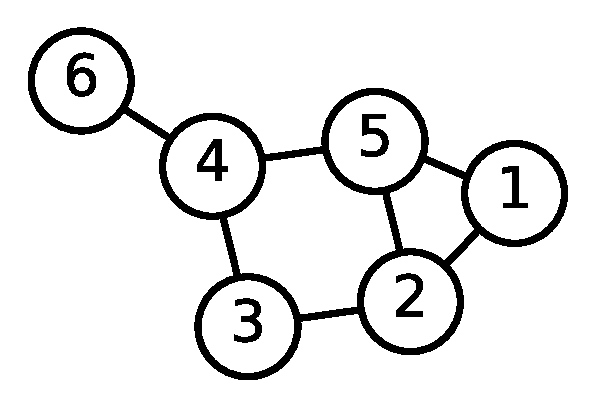
\includegraphics[width=3in]{connectivity.eps}
  \end{figure}
}
\frame
{
  \frametitle{Vertex cover -- Problem Statement}
  In the mathematical discipline of graph theory, a vertex cover of a graph is a set of vertices such that each edge of the graph is incident to at least one vertex of the set.
  \begin{block}{Formalized Definition}
  \begin{itemize}
  \item {\bf Input:} Graph $G$.
  \item {\bf Output:} Smallest number $k$ such that there is a vertex cover $C$ for $G$ of size $k$.
  \end{itemize}
  \end{block}
}
\frame
{
  \frametitle{Vertex cover -- Instance}
  \begin{figure}
  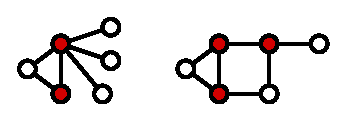
\includegraphics[width=3in]{Minimum-vertex-cover.eps}
  \end{figure}
}
\frame
{
  \frametitle{Shortest Path (no negative edge)}
  In graph theory, the shortest path problem is the problem of finding a path between two vertices (or nodes) such that the sum of the weights of its constituent edges is minimized. 
  \begin{block}{Formalized Definition}
  \begin{itemize}
  \item {\bf Input:} A weighted graph $G$ (that is, a set $V$ of vertices, a set $E$ of edges, and a real-valued weight function $f: E \rightarrow R^+$), two nodes $v$ and $v'$ of $V$
  \item {\bf Output:} A path $P$ from $v$ to $v'$ so that $\sum_{p \in P} f(p)$ is minimal among all paths connecting $v$ and $v'$.
  \end{itemize}
  \end{block}
}
\frame
{
  \frametitle{Shortest Path (no negative edge) -- Instance}
  \begin{figure}
  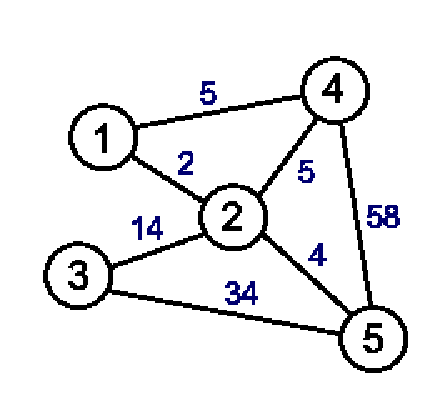
\includegraphics[width=2in]{wgraph.eps}
  \end{figure}
}
\frame
{
  \frametitle{Shortest Path (negative cycle)}
  In a weighed graph, a negative cycle is a cycle whose sum of edge weights is negative.
  \begin{block}{Formalized Definition}
  \begin{itemize}
  \item {\bf Input:} A weighted directed graph $G$ (that is, a set $V$ of vertices, a set $E$ of edges, and a real-valued weight function $f: E \rightarrow R$)
  \item {\bf Output:} A closed path $P \subseteq E$, such that $\sum_{e \in P}f(e) < 0$.
  \end{itemize}
  \end{block}
}
\frame
{
  \frametitle{Shortest Path (negative cycle) -- Instance}
  \begin{figure}
  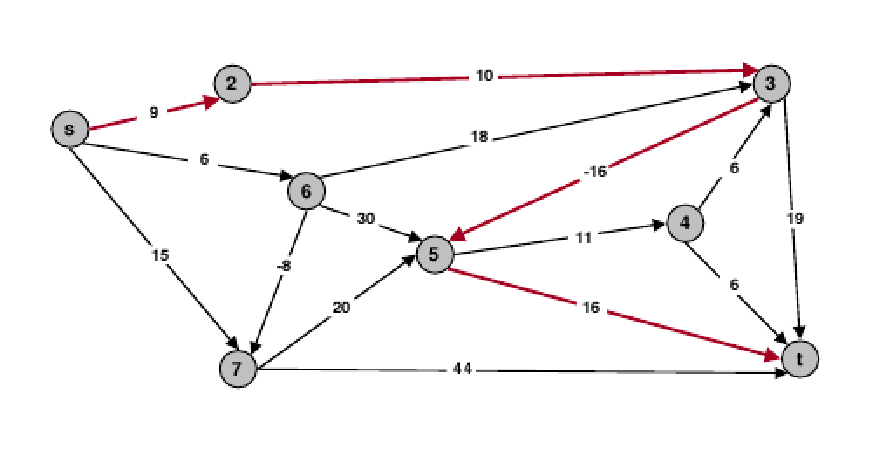
\includegraphics[width=3in]{negpath.eps}
  \end{figure}
}
\frame
{
  \frametitle{Merge Sort}
  Merge sort is an $O(n \log n)$ comparison-based sorting algorithm.
  \begin{block}{Formalized Definition}
  \begin{itemize}
  \item {\bf Input:} An array of numbers.
  \item {\bf Output:} A sorted array.
  \end{itemize}
  \end{block}
}
\frame
{
  \frametitle{Merge Sort -- Instance}
  Merge sort an array of 7 integers: 38, 27, 43, 3, 9, 82, 10.
  \begin{figure}
  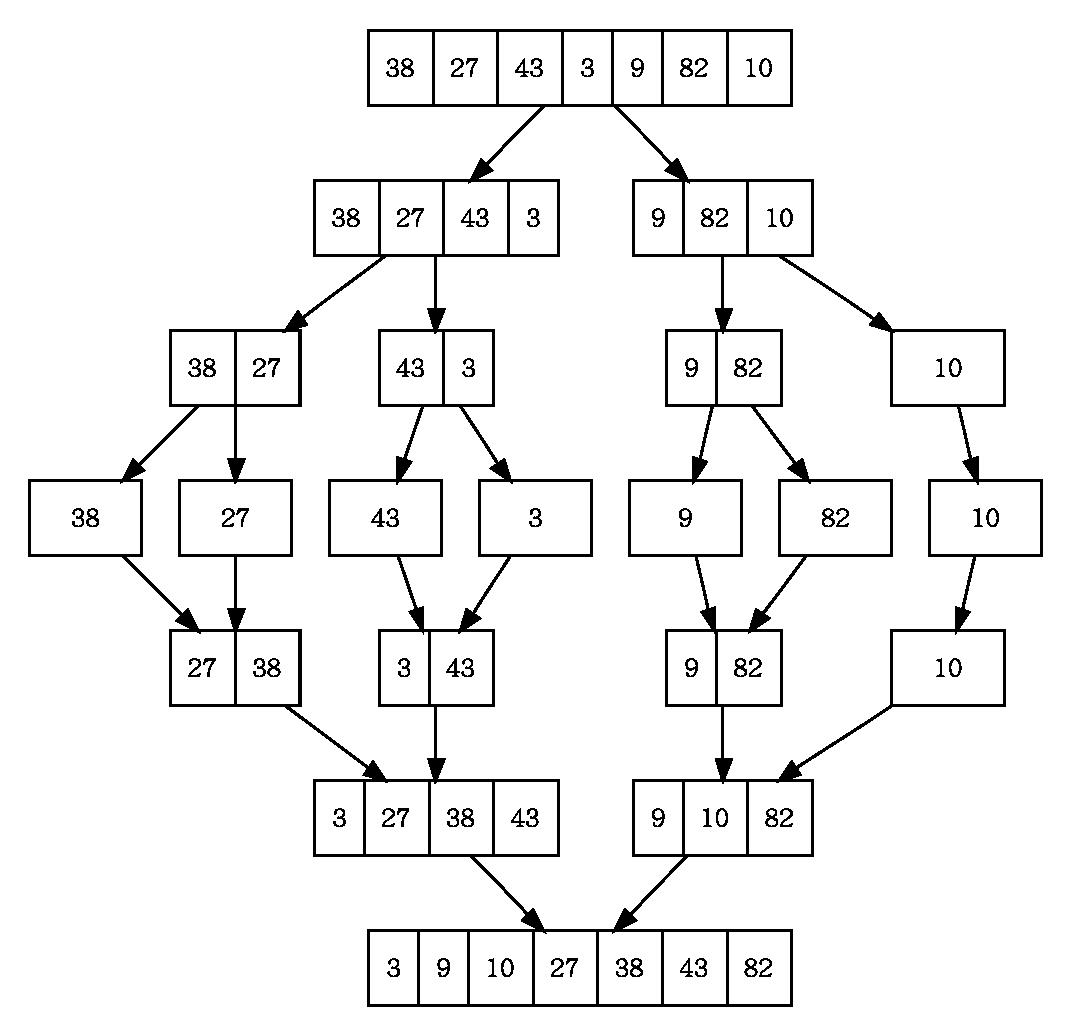
\includegraphics[width=3in]{Merge_sort.eps}
  \end{figure}
}
\frame
{
  \frametitle{RNA (SCFG)}
  A context-free grammar $G$ can be defined by $G = (V, T, P, S)$ where:
  \begin{itemize}
  \item V is a finite set of nonterminal symbols (`states'),
  \item T is a finite set of terminal symbols (for RNA: {a, c, g, u}),
  \item P is a finite set of production rules (described below), and
  \item S is the initial (start) nonterminal ($S \in V$).
  \end{itemize}
  \begin{block}{Formalized Definition}
  \begin{itemize}
  \item {\bf Input:} A sequence of terminal symbols.
  \item {\bf Output:} Second structure maximizing the number of base pairs.
  \end{itemize}
  \end{block}
}
\frame
{
  \frametitle{RNA (SCFG) -- Instance}
  \begin{figure}
  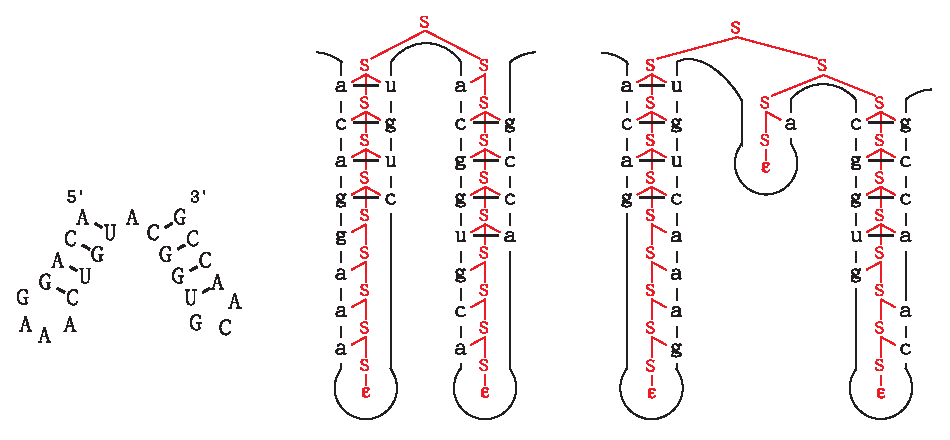
\includegraphics[width=3in]{SCFG.eps}
  \end{figure}
}

%%%%%%%%%%%%%%%%%%%%%%%%%%from here by Chunlin%%%%%%%%%%%%


\section{Minimum Convex Hull Problem}
\frame
{
\frametitle{Problem Statement}
The {\bf Convex Hull} of a set $Q$ of points is the smallest convex of polygon $P$ for which each point in $Q$ is either on the boundary of $P$ or in its interior.
\begin{block}{Formalized Definition:}
\begin{itemize}
    \item {\bf Input:} \\a set of points in the plane
    \item {\bf Output:}\\the convex hull of the points
\end{itemize}
\end{block}
}


\frame
{
\frametitle{Instance}
\begin{figure}
 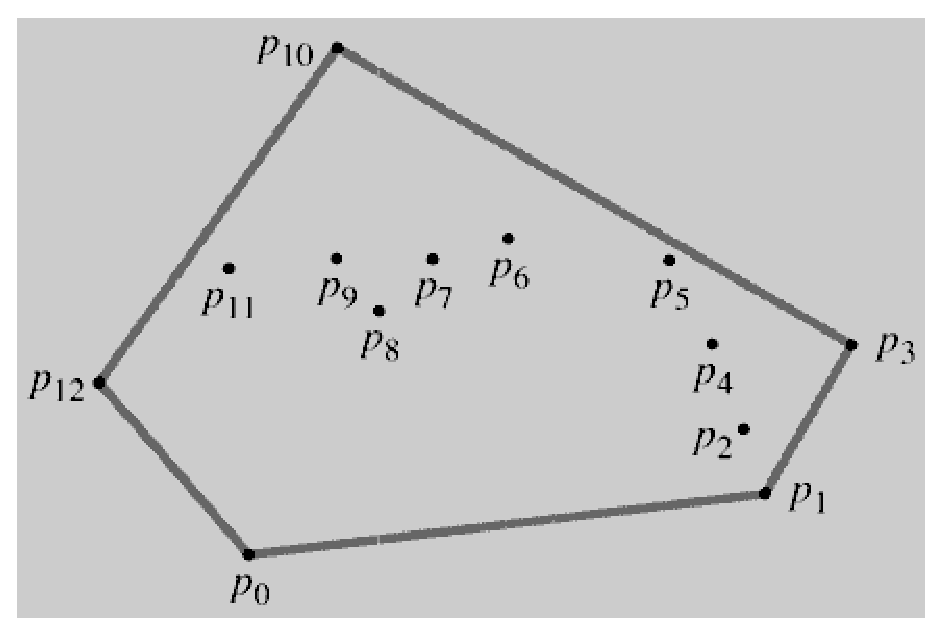
\includegraphics[width=3in]{example.eps}
\end{figure}

}

\frame
{
    \frametitle{Key Observation}
    \begin{itemize}
        \item Two Algorithms:
            \begin{itemize}
                \item Graham's Scan -- run in $O$($n$lg$n$) time
                \item Jarvis's March -- run in $O$($nh$) time
            \end{itemize}
        \item Both algorithms use a technique called \emph{rotational} sweep, which processing vertices in the order of the polar angles they form with a reference vertex.
     \end{itemize}
}


\section{Clustering Problem}
\frame
{
\frametitle{Problem Statement}
{\bf Clustering}, or \emph {cluster analysis}, is the assignment of a set of observations into subsets ( called \emph{clusters} ) so that observations in the same cluster are similar in some sense. It's a method of unsupervised learning, and a common technique for statistical data analysis used in many fields, including machine learning, data mining, pattern recognition, image analysis and bioinformatics. 
\begin{block}{Formalized Definition:}
	\begin{itemize}
		\item {\bf Input:}\\ a set of points in the plane
		\item {\bf Output:}\\ several clusters of the points, which make objects in different clusters far apart, while objects within the same cluster are close.
	\end {itemize}
\end{block}
}

%\section{Instance}
\frame
{
\frametitle{Instance}
\begin{figure}
	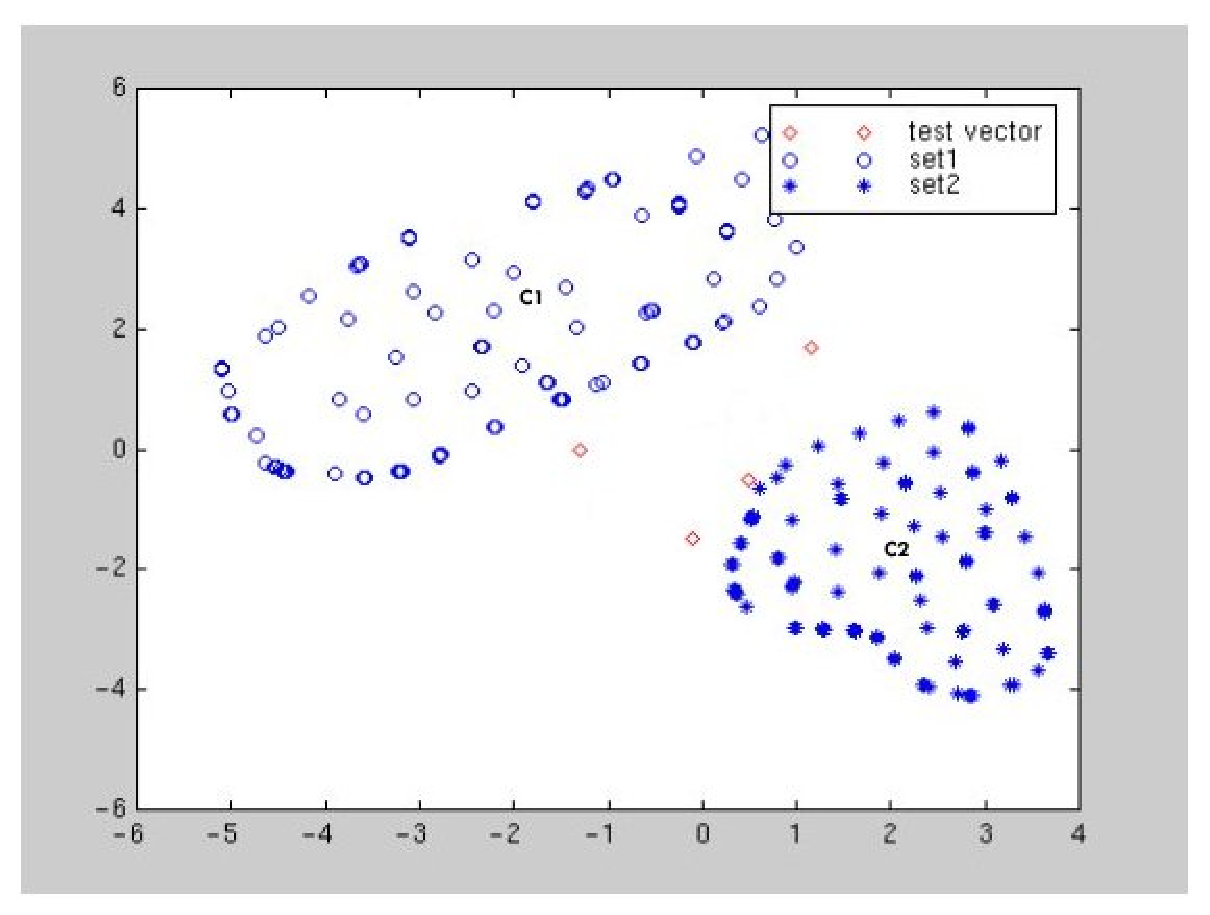
\includegraphics[width=2in]{KMeans.eps}
\end{figure}
\begin{center}
	A clustering problem settled by k-means algorithm
\end{center}
}

%\section{Key Observation}
\frame
{
\frametitle{Key Observation}
\begin{itemize}
	\item Distance Measure:\\
		    An important step in any clustering is to select a distance measure, which will determine how the similarity of two elements is calculated.\\
		eg. Euclidean Distance, Manhattan Distance, Hamming Distance, maximum norm
	\item Algorithms: How to efficiently find the one clustering that has maximum spacing?
		\begin{itemize}
			\item Greedy Algorithm: consider growing a graph on the vertex set and processing Kruskal's Minimum Spanning Tree Algorithm.
			\item Other ordinary algorithms: k-means clustering, fuzzy c-means clustering, QT clustering algorithm
		\end{itemize}
\end{itemize}
}

\section{KnapSack Problem}
\frame
{
\frametitle{Problem Statement}
Given a set of items, each with a weight and a value, determine the number of each item to include in a collection so that the total weight is less than a given limit and the total value is as large as possible.
\begin{block}{Formalized Definition:}
\begin{itemize}
    \item {\bf Input:}\\ a set of items $i$ with weight $w_i$ and value $v_i$, and a total weight limit $W$, $i$=1,2,\ldots,$n$
	\item {\bf Output:}\\ the set of items which maximize the total value with total weight below $W$
\end{itemize}
 %\begin{itemize}
 %\item {\bf Input:} \\a set of items $i$ with weight $w$_$i$ and value $v$_$i$, and a total weight limit $W$, $i$=1,2,\cdots,$n$
 %\item {\bf Output:}\\the set of items which maximize the total value with total weight below $W$
 %\end{itemize}
\end{block}
}

\frame
{
	\frametitle{Instance}
	\begin{center}
	What's the best solution?
	\end{center}
	\begin{figure}
	\includegraphics[width=2in]{486px-Knapsack.svg.eps}
	\end{figure}
}

\frame
{
	\frametitle{Instance}
	\begin{center}
	the best solution
	\end{center}
	\begin{figure}
	\includegraphics[width=2.3in]{1000px-Knapsack_greedy.svg.eps}
	\end{figure}
}

\frame
{
	\frametitle{Key Observation}
	\begin{itemize}
		\item The Subset-Sum($n$,$W$) Algorithm, using dynamic programming, correctly computes the optimal value of the problem, and runs in $O$($nW$) time. The problem is $NP$-hard and the algorithm is \emph{pseudo-polynomial}.
		\item We can design an improved algorithm, using approximation.
	\end{itemize}
}

\section{Global Minimum Cut Problem}
\frame
{
\frametitle{Problem Statement}
\begin{itemize}
	\item In this problem, we are given an undirected graph with positive weights on its edges, and we seek a proper subset $S$ of the vertices that minimizes the total weight of all edges that have exactly one endpoint in $S$.
	\item Another statement: Find the smallest total weight of edges whose deletion disconnects the undirected graph.
\end{itemize}
\begin{block}{Formalized Definition:}
	\begin{itemize}
		\item {\bf Input:} \\an undirected graph $G=(V,E)$, and every edge $e$ has a positive integer weight $w_e$
		\item {\bf Output:}\\the smallest total weight of edges whose deletion disconnects $G$
	\end{itemize}
\end{block}
}

\frame
{
\frametitle{Instance}
\begin{figure}
	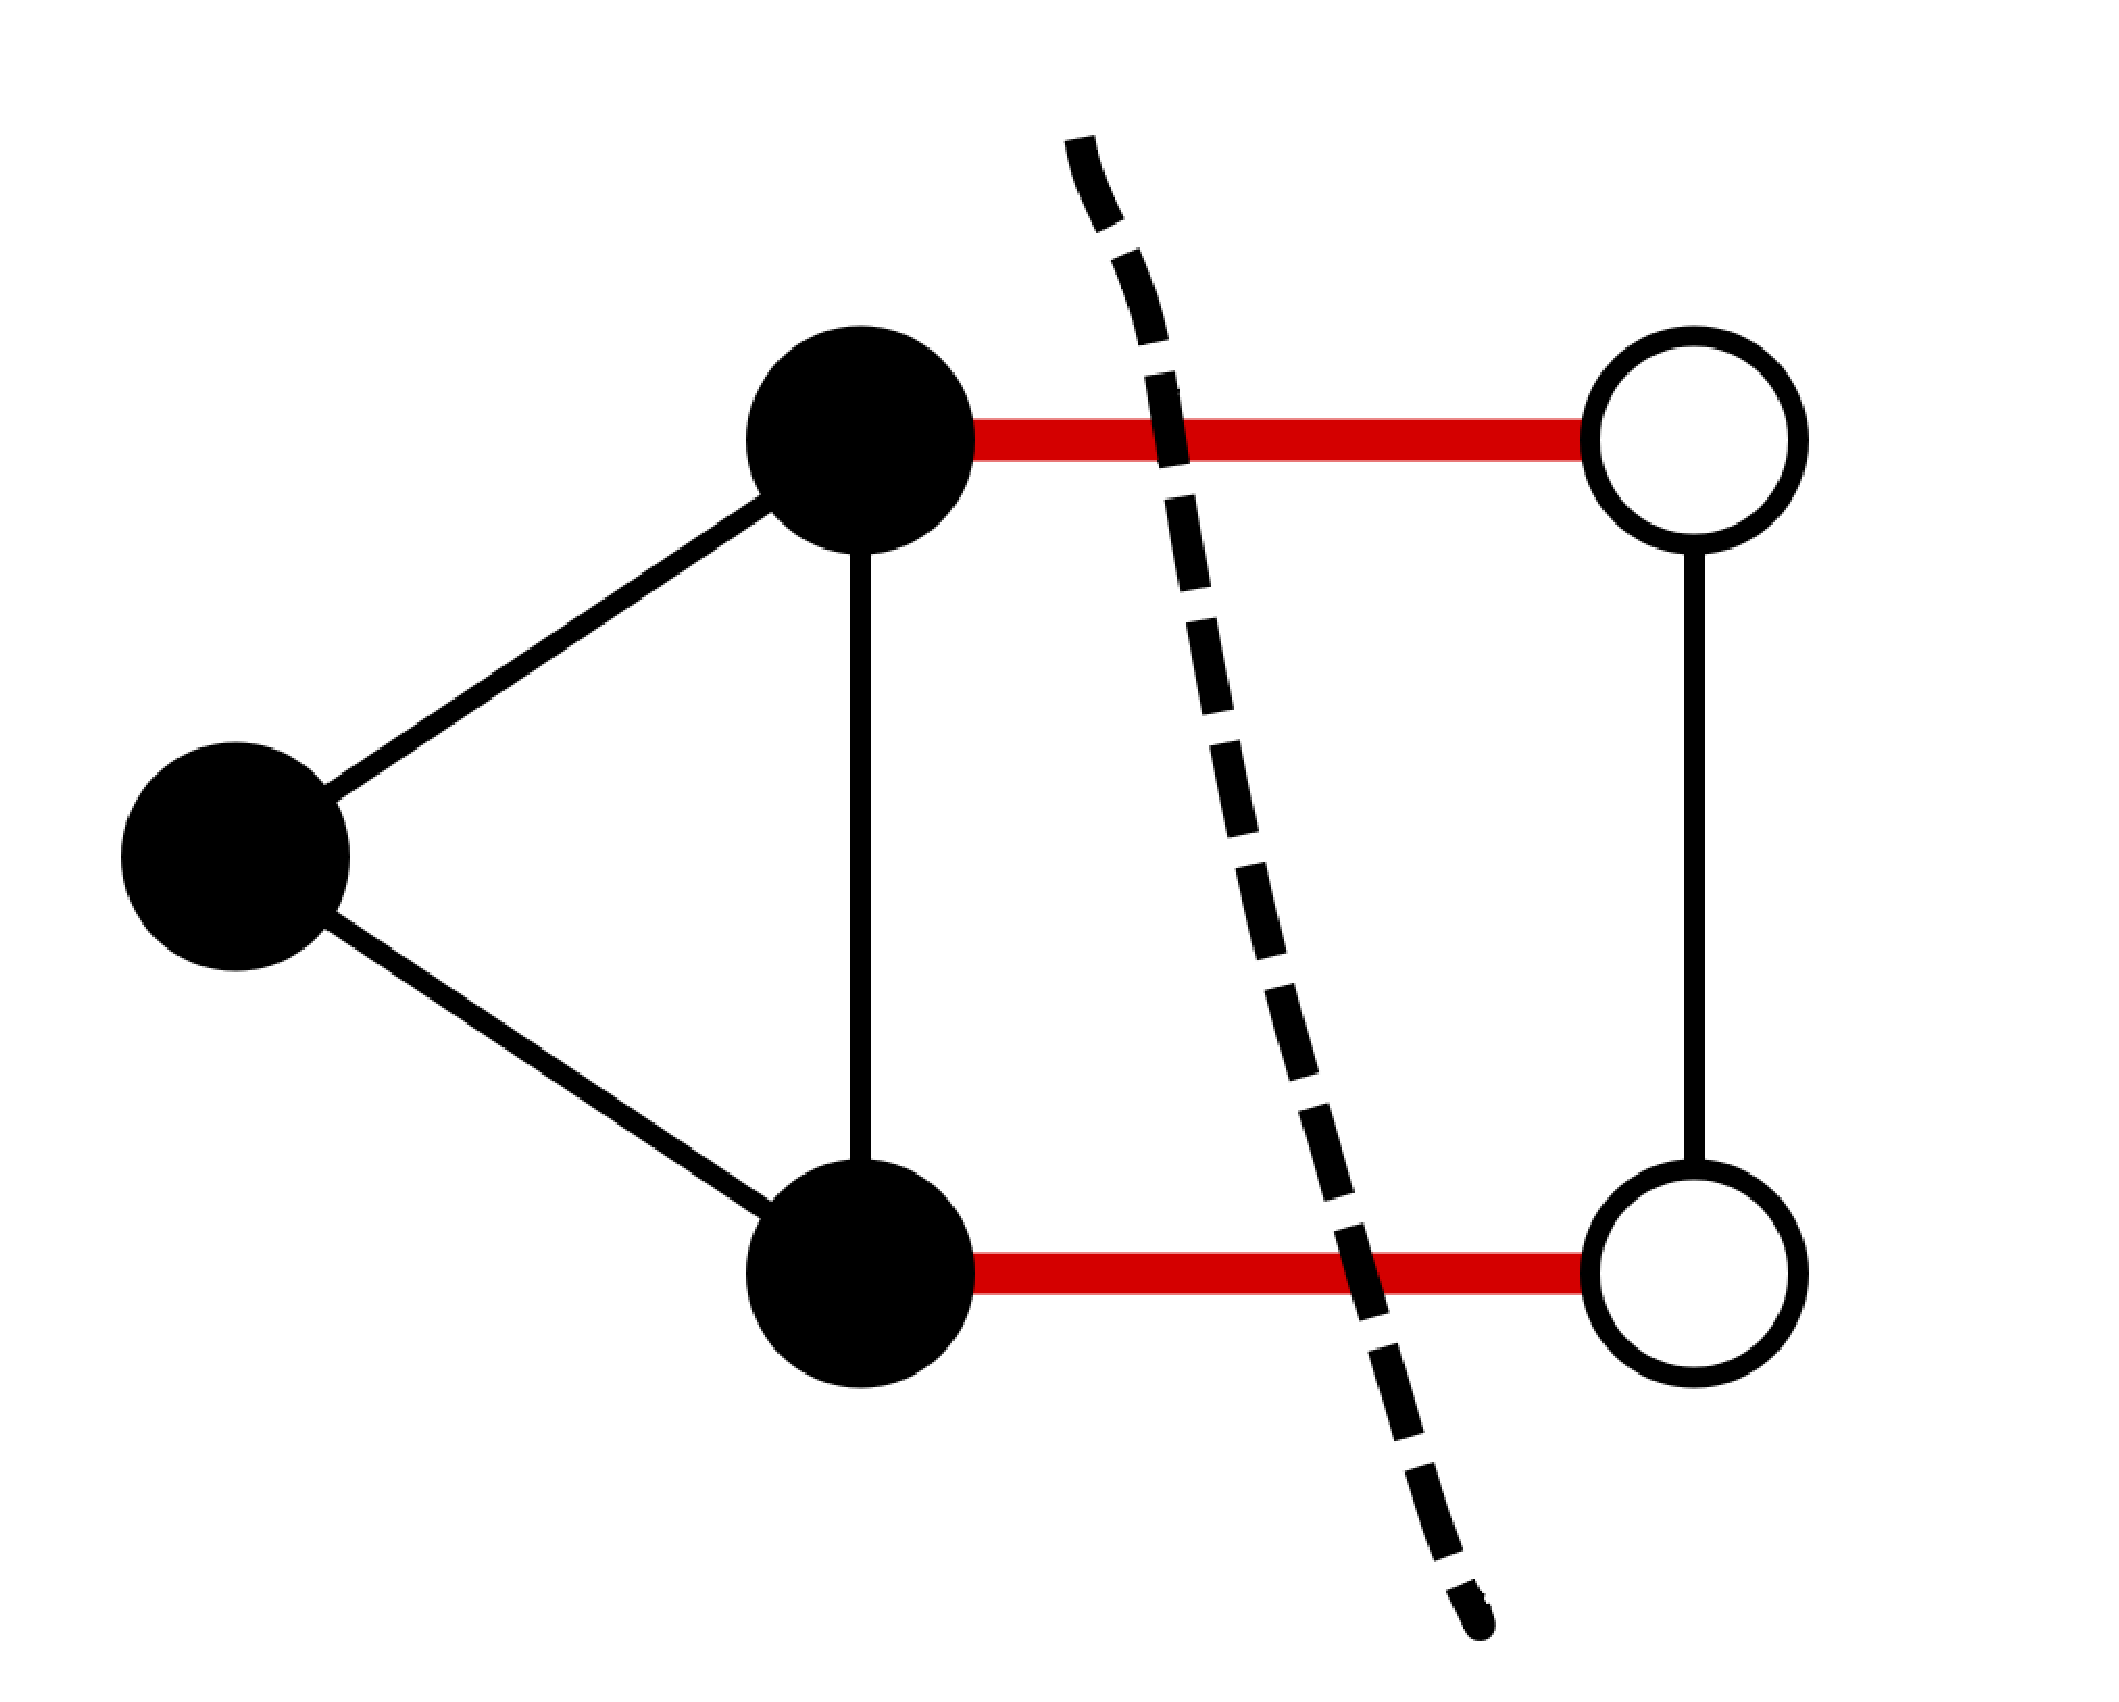
\includegraphics[width=2.5in]{1000px-Min-cut.svg.eps}
\end{figure}
}

\frame
{
\frametitle{Key Observation}
\begin{itemize}
	\item The \emph{max-flow min-cut theorem} states that the maximum value of an s-t flow is equal to the minimum capacity of an s-t cut.
	\item Or we can use the Contraction Algorithm, a kind of randomized algorithm, to solve the problem.
\end{itemize}
}

\section{Local Maximum Cut Problem}
\frame
{
\frametitle{Problem Statement}
\begin{itemize}
	\item For a graph, a \emph{maximum cut} is a cut whose size is not smaller than the size of any other cut. The problem of finding a maximum cut in a graph is known as the max-cut problem.
	\item Or, one wants a subset $S$ of the vertex set such that the total weight of edges between $S$ and the complementary subset is as large as possible.
\end{itemize}
\begin{block}{Formalized Definition:}
	\begin{itemize}
		\item {\bf Input:} \\an undirected graph $G=(V,E)$, and every edge $e$ has a positive integer weight $w_e$
		\item {\bf Output:}\\a partition $(A,B)$ of the vertex set so that $w(A,B)$ is maximized, and $w(A,B)=\Sigma_{e=\{ u,v\} ,u\in A,v\in B} w_e$
	\end{itemize}
\end{block}
}

\frame
{
\frametitle{Instance}
\begin{figure}
	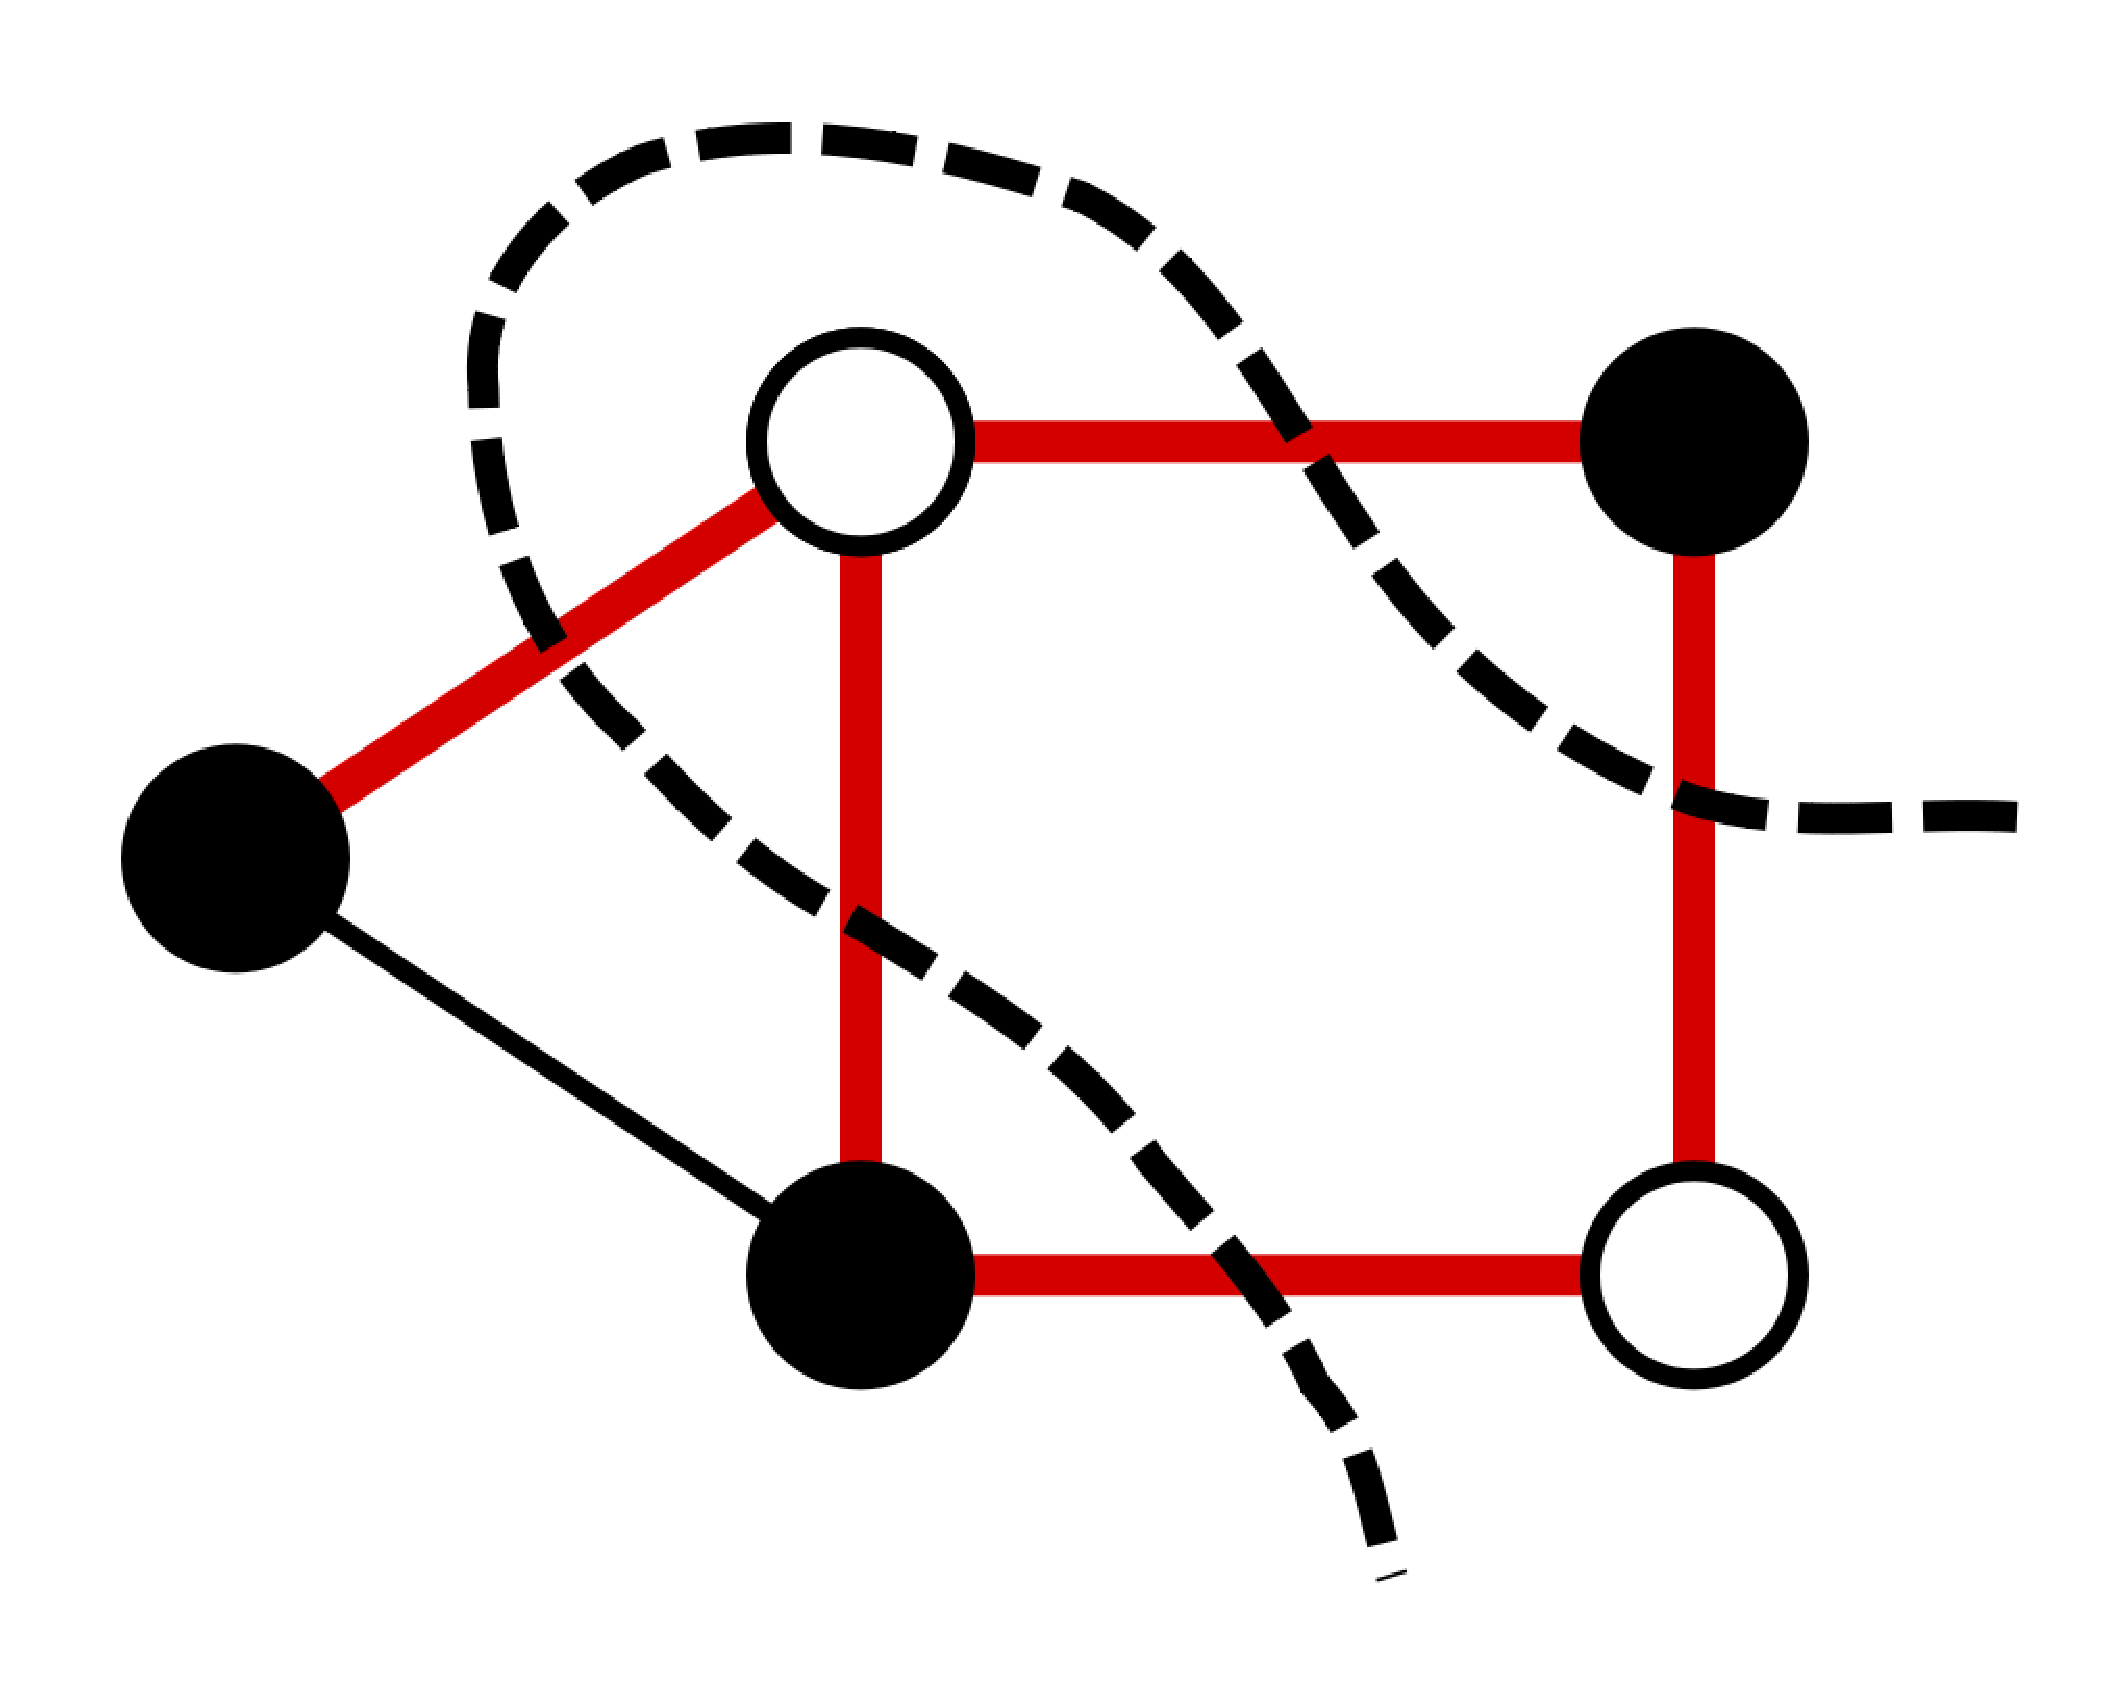
\includegraphics[width=1.7in]{1000px-Max-cut.svg.eps}
	\\
	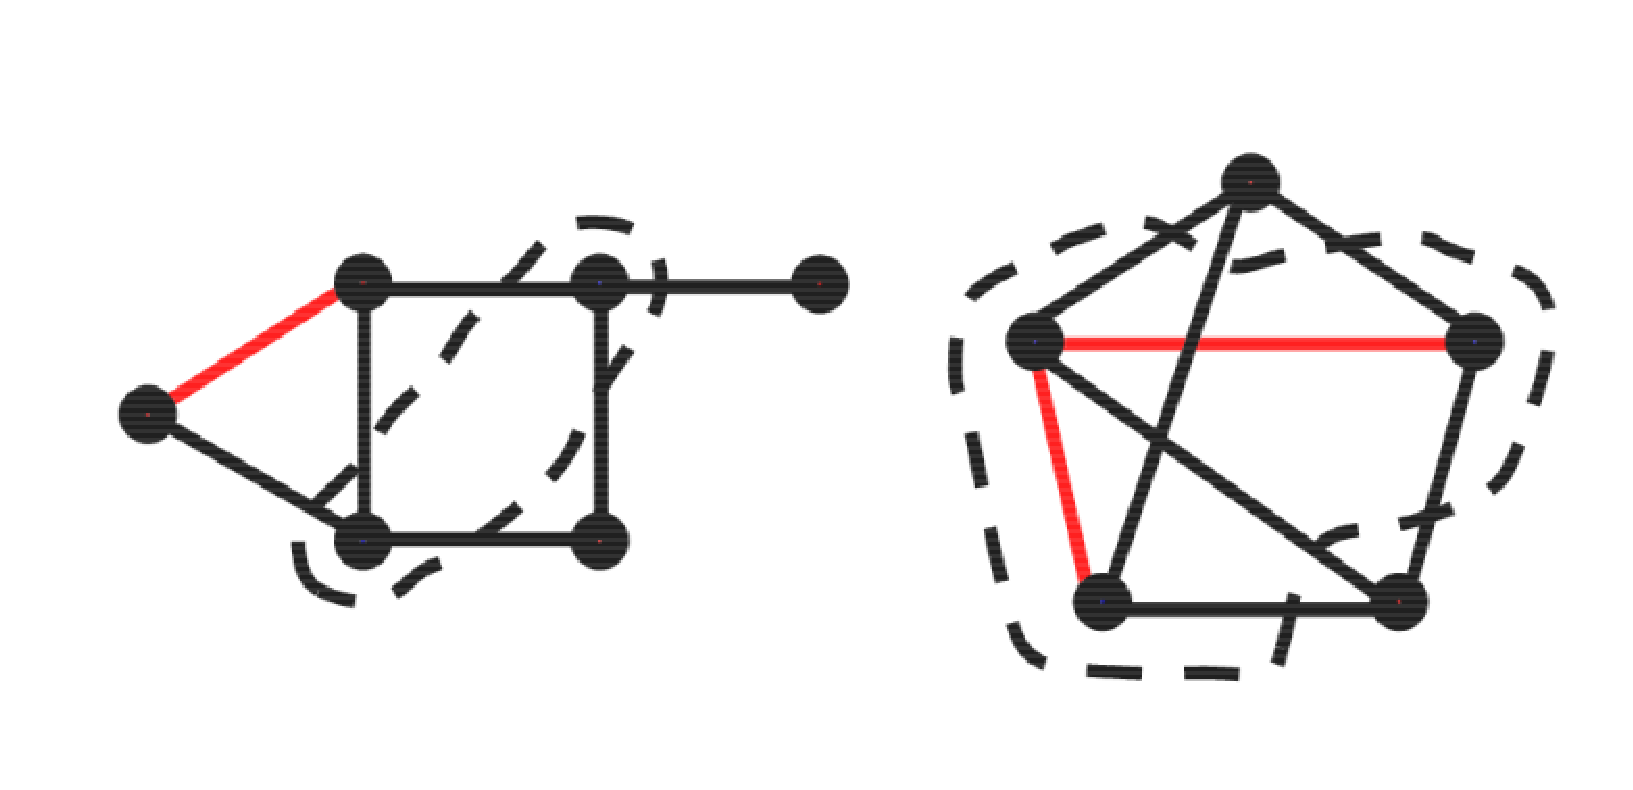
\includegraphics[width=2.8in]{maxcut_example_2.eps}
\end{figure}
}

\frame
{
\frametitle{Key Observation}
\begin{itemize}
	\item Maximum Cut is NP-hard.
	\item The State-Flipping Algorithm used for Hopfield networks provides a local search algorithm to approximate the Maximum Cut objective function.
\end{itemize}
}

%%%%%%%%%%%%%%%%%from here by Mingfu%%%%%%%%%%%%%%%%%%%

\section{SAT(Boolean Satisfiability Problem)}

\frame[allowframebreaks]
{
	\frametitle{\secname}
	\begin{block}{Definitions}
	A {\bf literal} is either a variable or the negation of a {\bf variable}.\\
	A {\bf clause} is a disjunction of literals.\\
	A {\bf formula} is in {\bf conjunctive normal form (CNF)} if it is a conjunction of clauses.
	\end{block}

	\begin{block}{Description}
	{\bf Input: } a CNF\\
	{\bf Output: } \emph{true} or \emph {false}. \emph{true} if and only if there exits some assignment 
	of TRUE and FALSE values to the variables that will make the entire formula true.
	\end{block}

	\begin{block}{Example}
	\begin{center}
	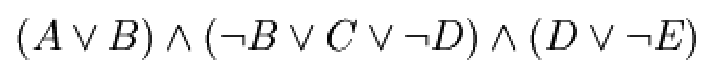
\includegraphics[width=0.7\textwidth]{p1.eps}
	\end{center}
	\end{block}

	\begin{block}{Observation}
	\begin{itemize}
	\item Complexity of \emph{enumeration} is $O(m2^n)$ while $n$ is the number of variables and $m$ is the number of clauses.
	\item The Cook-Levin theorem proves tha SAT is NP-complete: it was the first known NP-complete problem.
	\end{itemize}
	\end{block}
}

\section{Sum-free Set Problem}
\frame[allowframebreaks]
{
	\frametitle{\secname}
	\begin{block}{Definition}
	$A$ is sum-free if the equation $a+b=c$ has no solution with $a, b, c \in A$.
	\end{block}

	\begin{block}{Problem}
	How many sum-free subsets of $\{1,\cdots, n\}$ are there, for an integer $n$?
	\end{block}

	\begin{block}{Example}
	\begin{itemize}
	\item The sum-free sets of $\{1,2,3\}$ are $\emptyset$, $\{1\}, \{2\}, \{3\}, \{1,3\}$, and $\{2,3\}$. \\
	\item The numbers of sum-free subsets of $\{1,2,\cdots,n\}$ for $n=0, 1, \cdots$ are $1, 2, 3, 6, 9, 16, 24, 42, 61, \cdots$
	\end{itemize}
	\end{block}


	\begin{block}{Observation}
	\begin{itemize}
	\item Complexity of \emph{enumation} is $O(2^n)$.
	\item The answer has been shown to be $O(2^{N / 2})$, as predicted by the Cameron-Eros conjectur
	(proved by Ben Green and independently by Alexander Sapozhenko in 2003).
	\end{itemize}
	\end{block}
}

\section{Subset Sum Problem}
\frame
{
	\frametitle{\secname}
	\begin{block}{Description}
	{\bf Input: } A set of integers $S$\\
	{\bf Output: } \emph{true} or \emph{false}. 
	\emph{true} if there exists a subset $U$ of $S$ satisfying that the sum of elements of $U$ equals $0$.
	\end{block}

	\begin{block}{example}
	Given the set $\{ −7, −3, −2, 5, 8\}$, the answer is \emph{true} because the subset $\{ −3, −2, 5\}$ sums to zero.
	\end{block}

	\begin{block}{Observation}
		\begin{itemize}
			\item Complexity of \emph{enumation} is $O(n2^n)$, $n=|S|$.
		\end{itemize}
	\end{block}
}

\section{Huffman coding Problem}
\frame[allowframebreaks]
{
	\frametitle{\secname}
	\begin{block}{Descirption}
	{\bf Input: \\} 
	\begin{itemize}
	\item Alphabet $A = \left\{a_{1},a_{2},\cdots,a_{n}\right\}$, which is the symbol alphabet of size n.
	\item Set $W = \left\{w_{1},w_{2},\cdots,w_{n}\right\}$, which is the set of the symbol weights.
	\end{itemize}
	{\bf Output: } Code $C \left(A,W\right) = \left\{c_{1},c_{2},\cdots,c_{n}\right\}$,
		where $c_i$ is the codeword for $a_{i}, 1 \leq i \leq n$, 
		satisfying that $L\left(C\right) = \sum_{i=1}^{n}{w_{i}\times\mathrm{length}\left(c_{i}\right)}$ is the smallest. 
	\end{block}

	\begin{block}{Example}
	\begin{center}
	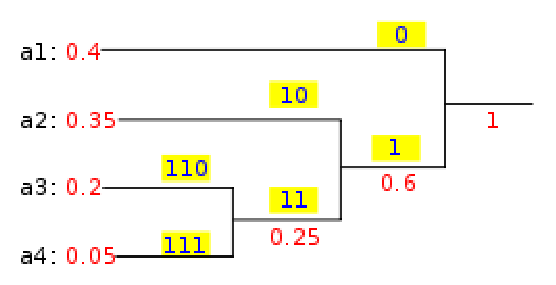
\includegraphics[width=0.4\textwidth]{p4.eps}
	\end{center}
	\end{block}

	\begin{block}{Observation}
	\begin{itemize}
	\item {\bf Shannon's source coding theorem:} the \emph{entropy} of $A$, $H(A) =  - \sum_{i=1}^n w_i \log_2 w_i$,
		is a measure of the smallest codeword length that is theoretically possible for the given alphabet with associated weights.
	\item algorithm : binary tree.
	\end{itemize}
	\end{block}
}

\section{Alignment Problem}
\frame[allowframebreaks]
{
	\frametitle{\secname}
	\begin{block}{Description}
	{\bf Input: } 2 sequences $S_1$ and $S_2$\\
	{\bf Output: } a mapping from $S_1$ to $S_2$ allowing \emph{insert} and \emph{delete} to make the \emph{scoring function} smallest.
	\end{block}

	\begin{block}{Example}
		\begin{center}
			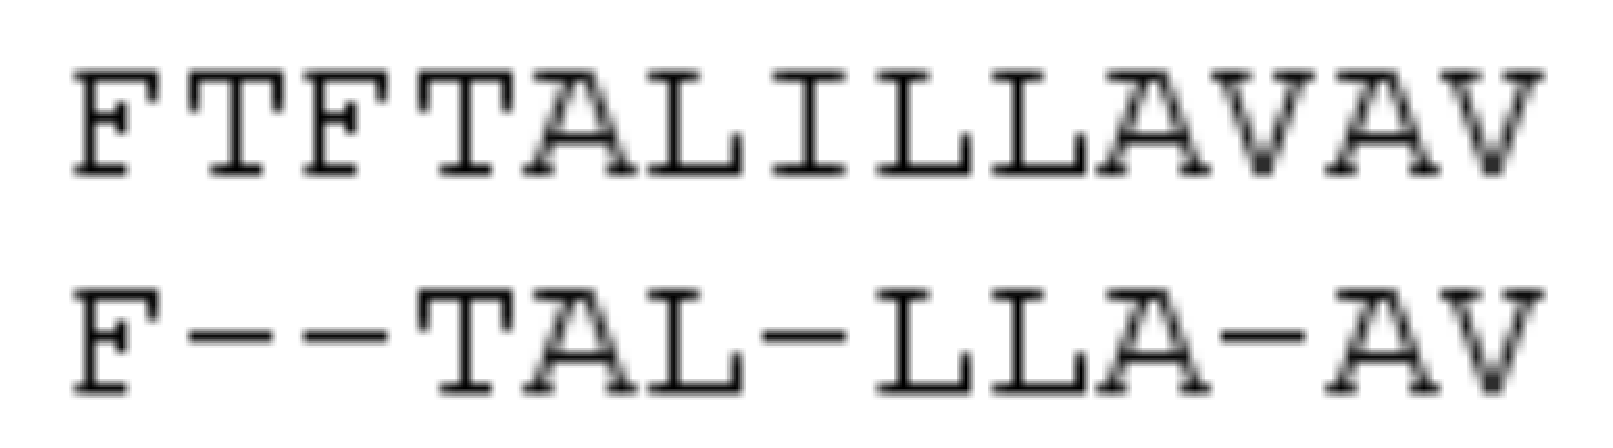
\includegraphics[width=0.5\textwidth]{p51.eps}
		\end{center}
		\begin{center}
			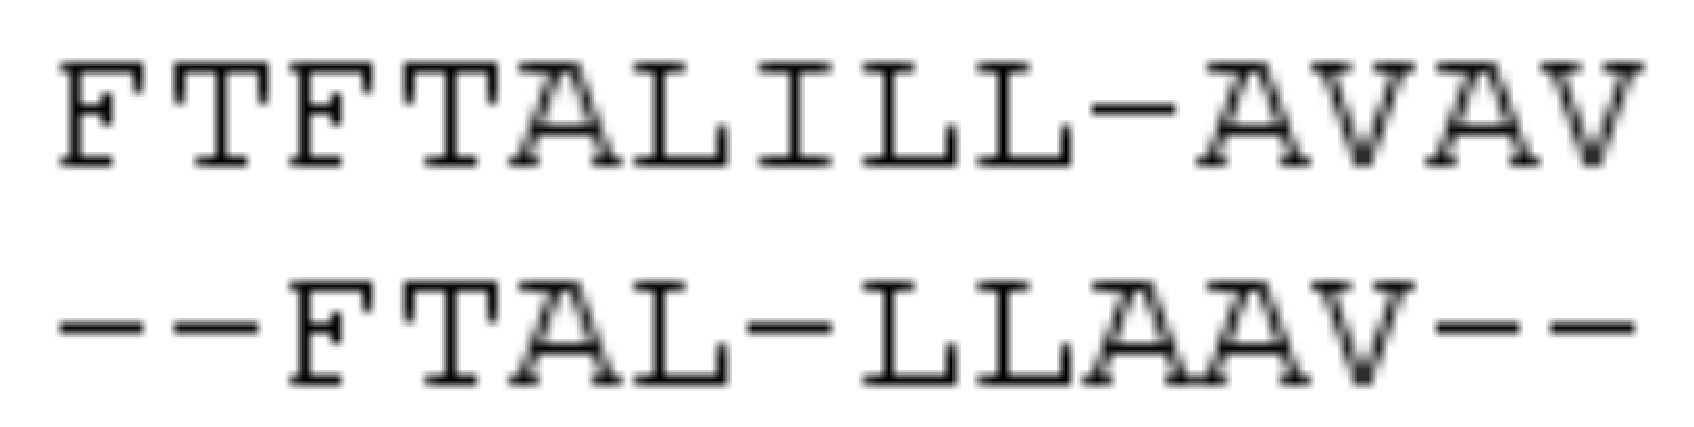
\includegraphics[width=0.5\textwidth]{p52.eps}
		\end{center}

	\end{block}

	\begin{block}{Obervation}
	\begin{itemize}
	\item Dynamic Programming algorithm
	\end{itemize}
	\end{block}
}


\section{Center Selection Problem}
\frame[allowframebreaks]
{
	\frametitle{\secname}
	\begin{block}{Description}
	{\bf Input: } $n$ sites $s_1, s_2, \cdots, s_n$, integer $k$\\
	{\bf Output: } $k$ centers satifying that maximum distance from a site to its nearest center is minimized.
	\end{block}

	\begin{block}{Example}
	\end{block}

	\begin{block}{Obervation}
	\begin{itemize}
	\item greedy(approximate algorithm)
	\end{itemize}
	\end{block}
}
%%%%%%%%%%%%%%%%%%%%%from here by Haicang%%%%%%%%%%%%%%%

\frame
{
\frametitle{Traveling Salesman Problem -- Problem Statement}
 $Traveling \ Salsesman \ Problem$ is one of the most famous sequencing problems in theoretical computer science.Given a list of cities and their pairwise distances,
the task is to find a shortest possible tour that visits each city exactly once.
\begin{block}{Formalized Definition:}

Input: \\

A directed gragh(The "directed" means that it may happen that $d(v_i,v_j) \  \neq \ d(v_j,v_i))$.The reason for this is to make our formulaiton as general as possible.) and a bound  $D$\\

Output: 
\begin{itemize}
 \item $1$ if there exits a tour of length at most $D$.
 \item $0$ for others.
\end{itemize}

\end{block}
}
\frame
{
\frametitle{Traveling Salesman Problem -- Instance}

\begin{figure}
 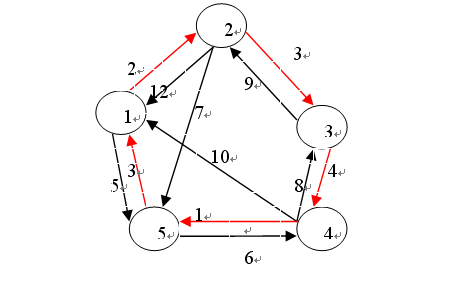
\includegraphics[width=3in] {tsp1.eps}
 % tsp1.eps: 22002048x0 pixel, 300dpi, 186284.00x0.00 cm, bb=14 14 407 318
\end{figure}

The tour path with the shortest length is  $1, \ 2, \ 3, \ 4, \ 5, \ 1$ with red color. 

}


\frame
{
\frametitle{Traveling Salesman Problem -- Key to the problem}
\begin{itemize}
 \item This problem has been proved an $NP$ problem.
 \item A trivial method : Enumerate. The time complexity will be $O(N!)$ , in which $N$ means the number of the vertice.
 \item For some special cases, when $N$ is very small,Various Branch-And-Bound algorithm.
 \item Heuristics and Approximation Algorithms, which quickly yield good solutions can be devised.
\end{itemize}

}
\frame
{
\frametitle{Set Cover Problem -- Problem Statement}
$Set \ Cover  \ Problem$ is a classical question in computer science and complexity theory. As input you are given several sets. They may have some elements in common. You must select a minimum number of these sets so that the sets you have picked contain all the elements that are contained in any of the sets in the input.
\begin{block}{Formalized Definition:} 
\begin{itemize}
 \item Input: 
A set $U$ of $n$ elements,a collection $S_1, S_2,...,S_m$ of subsets of $U$, and a number $k$.

 \item Output: 
\begin{itemize}
  \item $1$ if there exits a collection of at most $k$ of these sets whose union is equal to all of $U$.
  \item $0$ for others.
\end{itemize}

\end{itemize}
\end{block}
}


\frame
{
\frametitle{Set Cover Problem -- Instance}
In this instance,there is a collection of three of the sets whose union is equal to all of $U$:We can choose the tall thin oval on the left ,together with the two ploygons.
\begin{figure}
 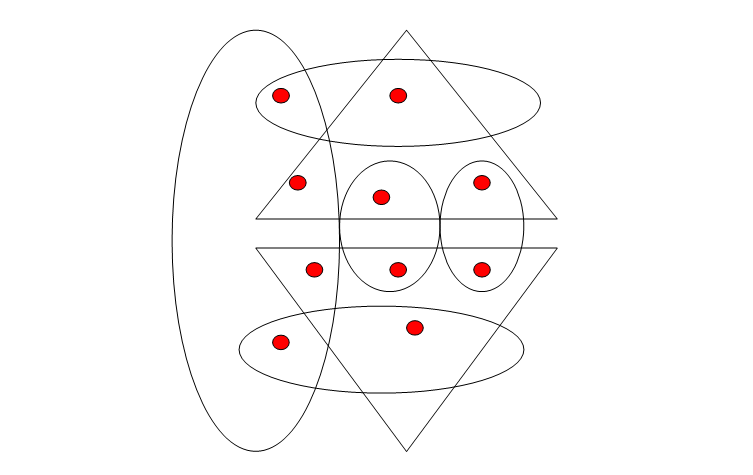
\includegraphics[width=3in]{setcover1.eps}
 % setcover1.eps: 22002048x0 pixel, 300 dpi, 186284.00x0.00 cm, bb=14 14 407 318
\end{figure}
In this instance,there is a collection of three of the sets whose union is equal to all of $U$:We can choose the tall thin oval on the left ,together with the two ploygons.
  


}


\frame
{
\frametitle{Set Cover Problem -- Key to the problem}
\begin{itemize}
 \item This problem has been proved an $NP$ problem.
 \item A trivial method : Enumerate. The time complexity will be $O(C^k_n)$ , in which $n$ means the number of the elements of the set $U$ and the  k means that at most of k subsets can be selected.
 \item The $Set \ Cover \ Problem $ can be formulated as the Integer Linear Program.
 \item Inapproximability results can be obtained by Approximation Algorithm 
\end{itemize}

}

\frame
{
\frametitle{Prime -- Problem Statement}
$Primality \ Test$ is an algorithm for determining whether an input number is prime. Amongst other fields of mathematics, it is used for cryptography. 
\begin{block}{Formalized Definition:}
\begin{itemize}
 \item Input: 
An positive integer $N$.

 \item Output: 
\begin{itemize}
  \item $1$ If $N$ is prime.
  \item $0$ for others.
\end{itemize}

\end{itemize}
\end{block}
}

\frame
{
\frametitle{Prime -- Instance}
\begin{block}{Instance}
\begin{itemize}
 \item $17$ is prime 
 \item $2^{42,643,801}-1$ is the largest known prime.
 \item $2^{2^7}$ is composite because $2^{2^7}$ = $5964958812749721*5704689200685129054721$
\end{itemize}

\end{block}

}
\frame
{


\frametitle{Prime -- Key to the problem}
\begin{itemize}
 \item A trivial method : check whether any integer i from 2 to $\sqrt{n}$ divides n.
 \item $Wilson's \ theorem$ states that $n$ is prime if and only if:
 $(n-1)!\ \equiv\ -1\ (\mbox{mod}\ n)$

Although this method is simple but it is inefficient and impratical because of modular multiplications.
 \item Randomized Algorithm has been used for $Primality \ Test$.
\end{itemize}

}


\end{document}

